\section{\textbf{Manufacturing}}\label{sec:4}
    For this project two PCB were made, hence in the presentation will be used two motors.
    As the simulation (see Section~\ref{sec:3}) proved that the designed circuit (see Figure~\ref{fig:schem}) works as intended the physical components were assembled in a breadboard for further testing and validation before the final manufacturing \todo{complete with relevant information about final board}. Figure~\ref{fig:proto_h} shows the circuit properly assembled. This circuit's evaluation will be further discussed in Section~\ref{sec:5}.

    \subsubsection{Fritizing} % (fold)
    \label{ssub:fritizing}
        For aid the design of the printed circuit board it was used the software Fritizing\footnote{\url{http://fritzing.org/}}, that is an open source software used worldwide by hobbyists and it is an Electronic Design Automation software.
        The software Fritizing has 3 environments, shown in Figure~\ref{fig:breadboard}, they are breadboard, schematic and PCB, it was used only the schematic and design environments since the breadboard already has been evaluated. The Figures~\ref{fig:schem_fritz} and~\ref{fig:pcb_fritz} show the schematics and PCB environments designing the board.
    % subsubsection fritizing (end)

    \subsubsection{Design} % (fold)
    \label{ssub:design}
        After tested on breadboard the H Bridge goes to design step were the components and PCB layout were chosen. The board have the following components:
        \begin{itemize}
            \item 1 switch with 3 states (on 1, off, on 2);
            \item 4 transistors NPN TIP31C;
            \item 4 resistors of $100\:\Omega$;
            \item 1 motor;
            \item 1 power source;
        \end{itemize}
        To interchange between the activation of Q1/Q2 and Q3/Q4 a switch component capable of turn on each side of the H bridge and turn off both sides was chosen, TIP31C was chosen because of its wide use range and readiness in buying. The resistors was the same as in the simulation and the motor chosen arbitrarily.
    % subsubsection printing (end)

    \subsubsection{Printing} % (fold)
    \label{ssub:printing}
        The H Bridge PCB was made on a CNC machine, which can be either milling as drill machine being able to made the circuit tracks and drill the components holes. The CNC machine is set at LARA, Figure~\ref{fig:workstation}, an ENE-UnB laboratory, and it has been used for prototyping PCBs. With the layout done in Fritizing the project was exported in a Geber extension(RS-274X) and then it was used the FlatCAM\footnote{\url{http://flatcam.org/}} software to read the Geber files and generate the G code of the path for the milling and drill tool. After setting the length of the tools, the CNC machine was calibrated and leveled, so it was started the PCB printing. The first version of the circuit gone through the continuity test, it was corrected some printing issues as tracks not fully separated, also the hole for the switch was too tight then it was used a Dremel to increase the radius. Finished the PCB test, the soldering had begun, the first components soldier was resistors as they're the less problematic components, followed by the transistors and then the headers for the power source and the motor. Due to an undesired current on the motor when the switch is turned off, a new version of the board was designed, printed and assembled, the new version has 4 new resistors connecting each transistor's base to the ground, the main value of this resistors are $1k\Omega$.
    % subsubsection printing (end)
	
	For the sake of validation the Magician Chassis (see Figure~\ref{fig:mag}) was properly assembled and each board produced was attached to a motor which was connected to a wheel of the Chassis. This allowed the vehicle to move forward or backward depending on the switch's position.

\begin{figure}[t]
\centering
\centering%
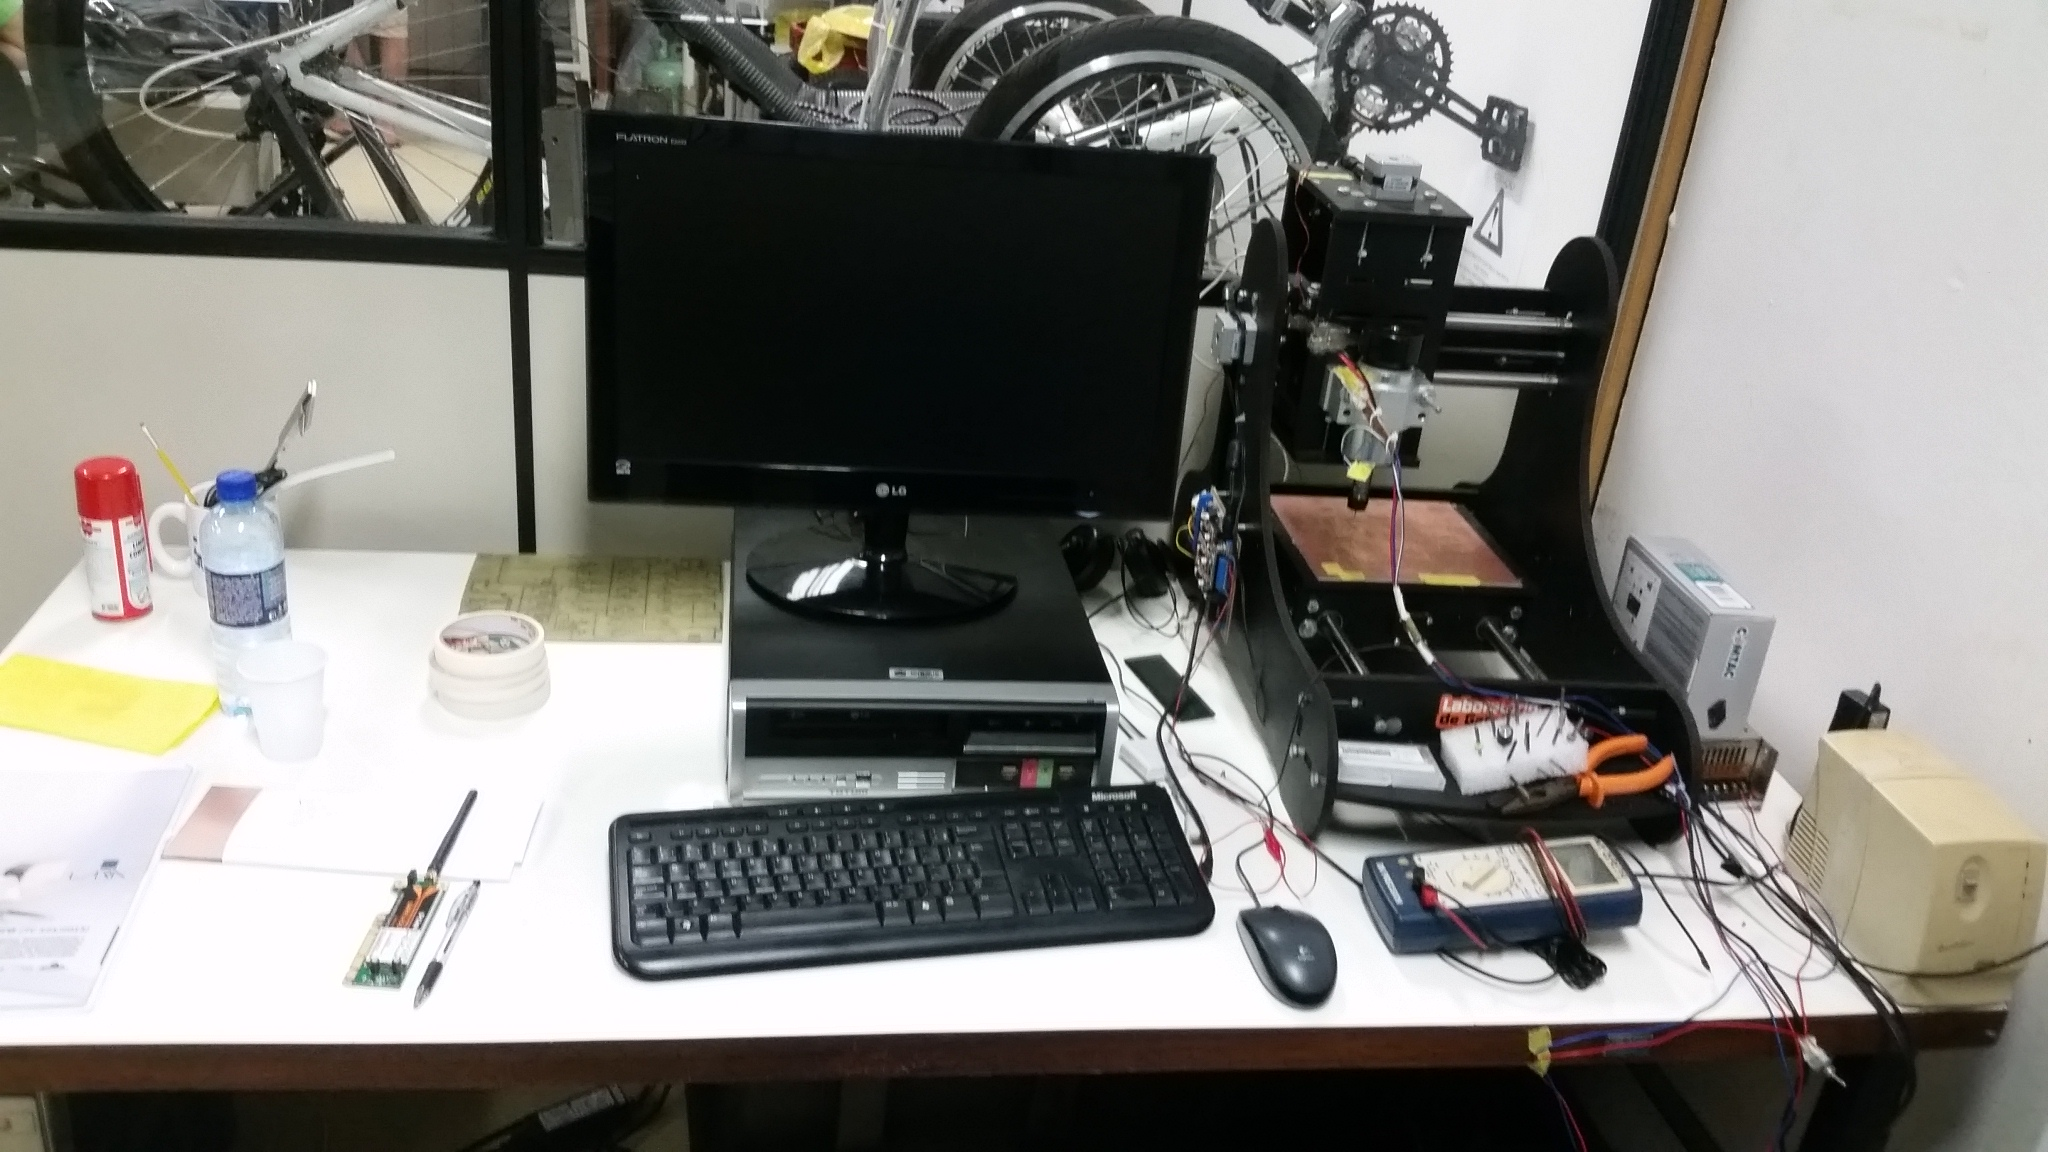
\includegraphics[height=.35\textwidth]{img/workstation_cnc.jpg}
\caption{CNC Workstation.}
\label{fig:workstation}%
\end{figure}

\begin{figure}[t]
\centering
\centering%
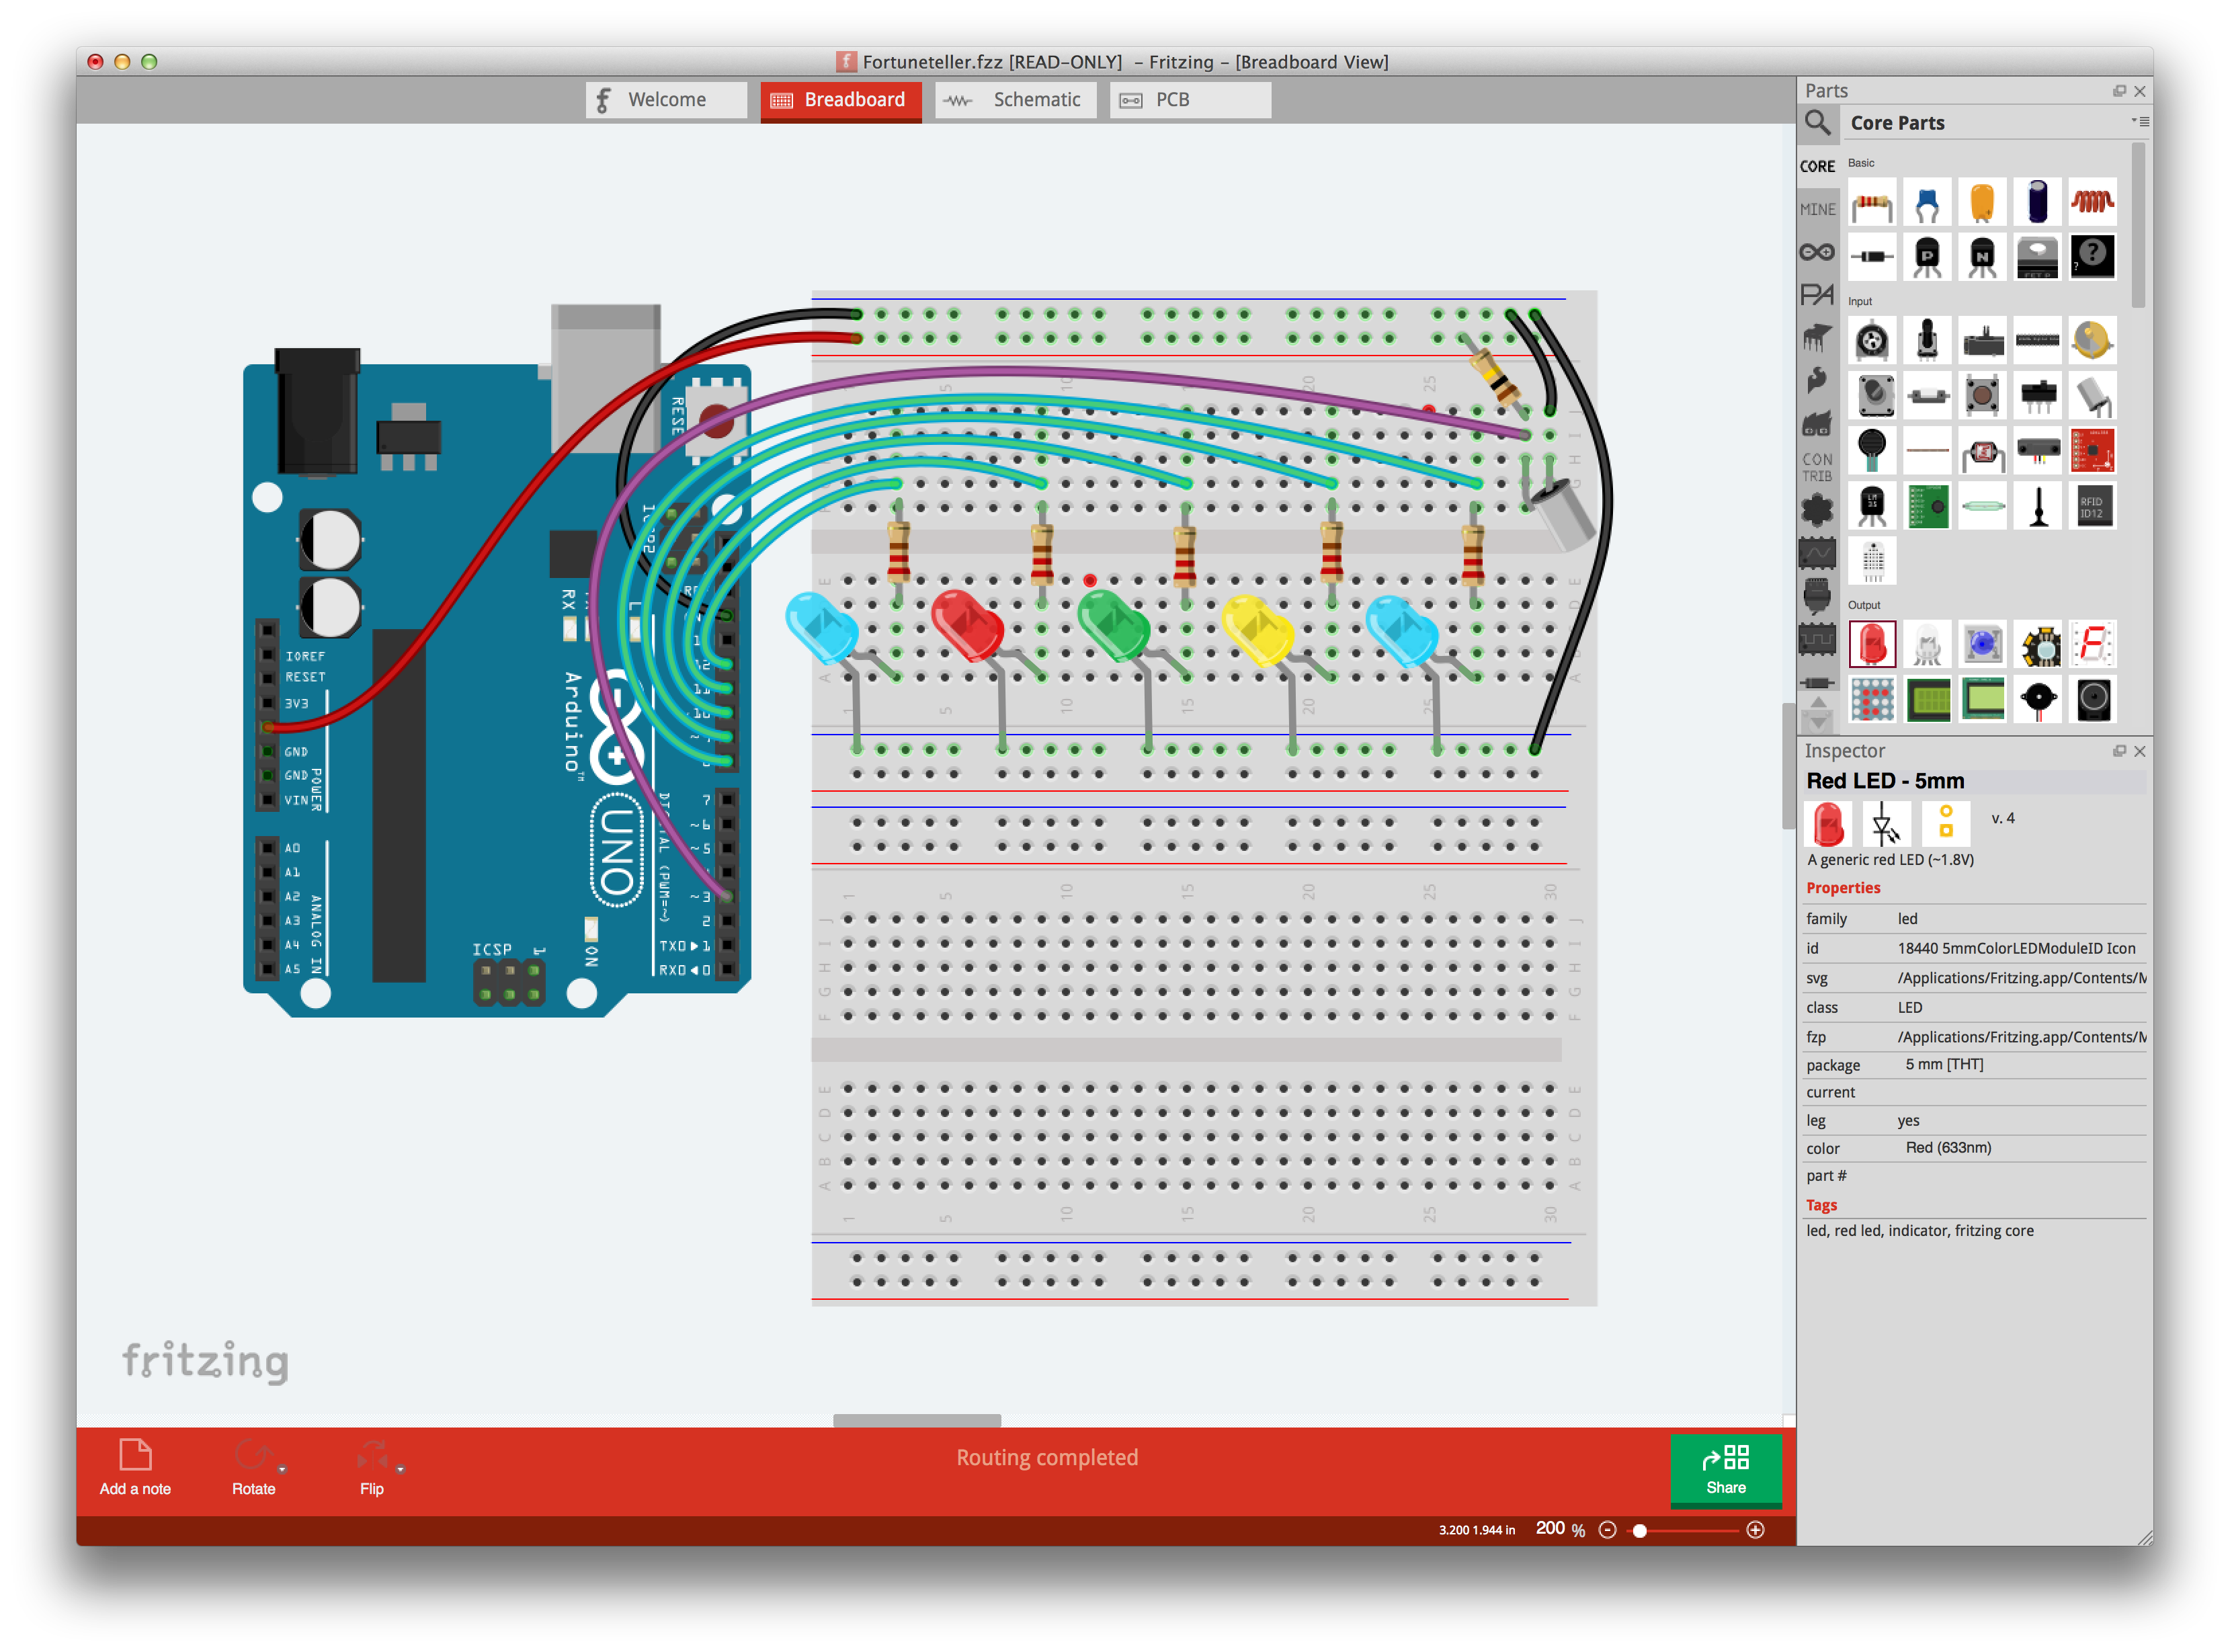
\includegraphics[height=.35\textwidth]{img/FritzingBreadBoard.png}
\caption{Fritizing showing the breadboard environment.}
\label{fig:breadboard}%
\end{figure}

\begin{figure}[t]
\centering
\centering%
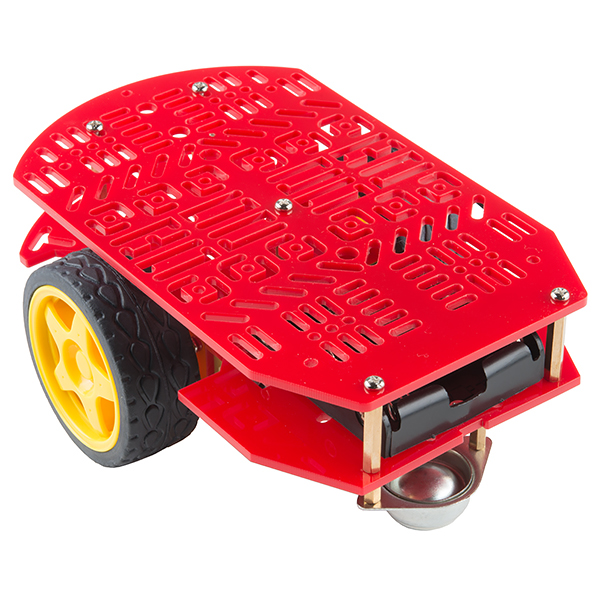
\includegraphics[height=.35\textwidth]{img/magician.jpg}
\caption{Magician Chassis (picture borrowed from Sparkfun site).}
\label{fig:mag}%
\end{figure}

\begin{figure}
\centering
\begin{subfigure}{\columnwidth}
\centering
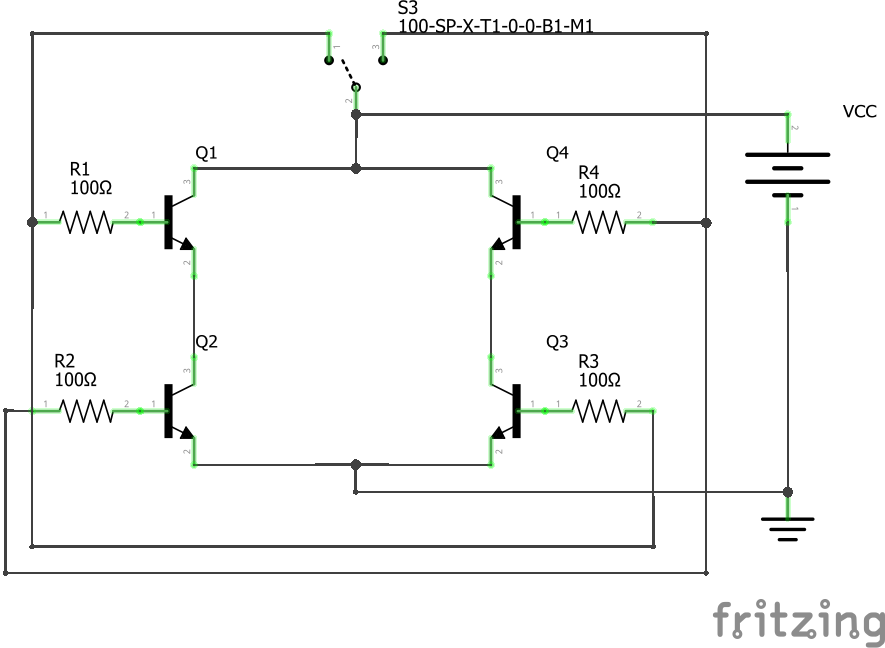
\includegraphics[height=.65\textwidth]{img/ponteH_schem.png}
\caption{Schematic on Fritizing.}
\label{fig:schem_fritz}
\end{subfigure}

\begin{subfigure}{\columnwidth}
\centering
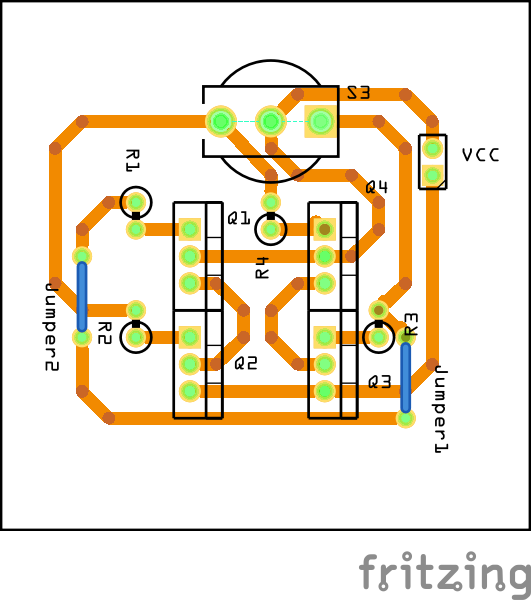
\includegraphics[height=.75\textwidth]{img/ponteH_pcb.png}
\caption{PCB design on Fritizing.}
\label{fig:pcb_fritz}
\end{subfigure}

\caption{H Bridge on Fritizing.}
\end{figure}


\begin{figure}
\centering
\begin{subfigure}{\columnwidth}
\centering
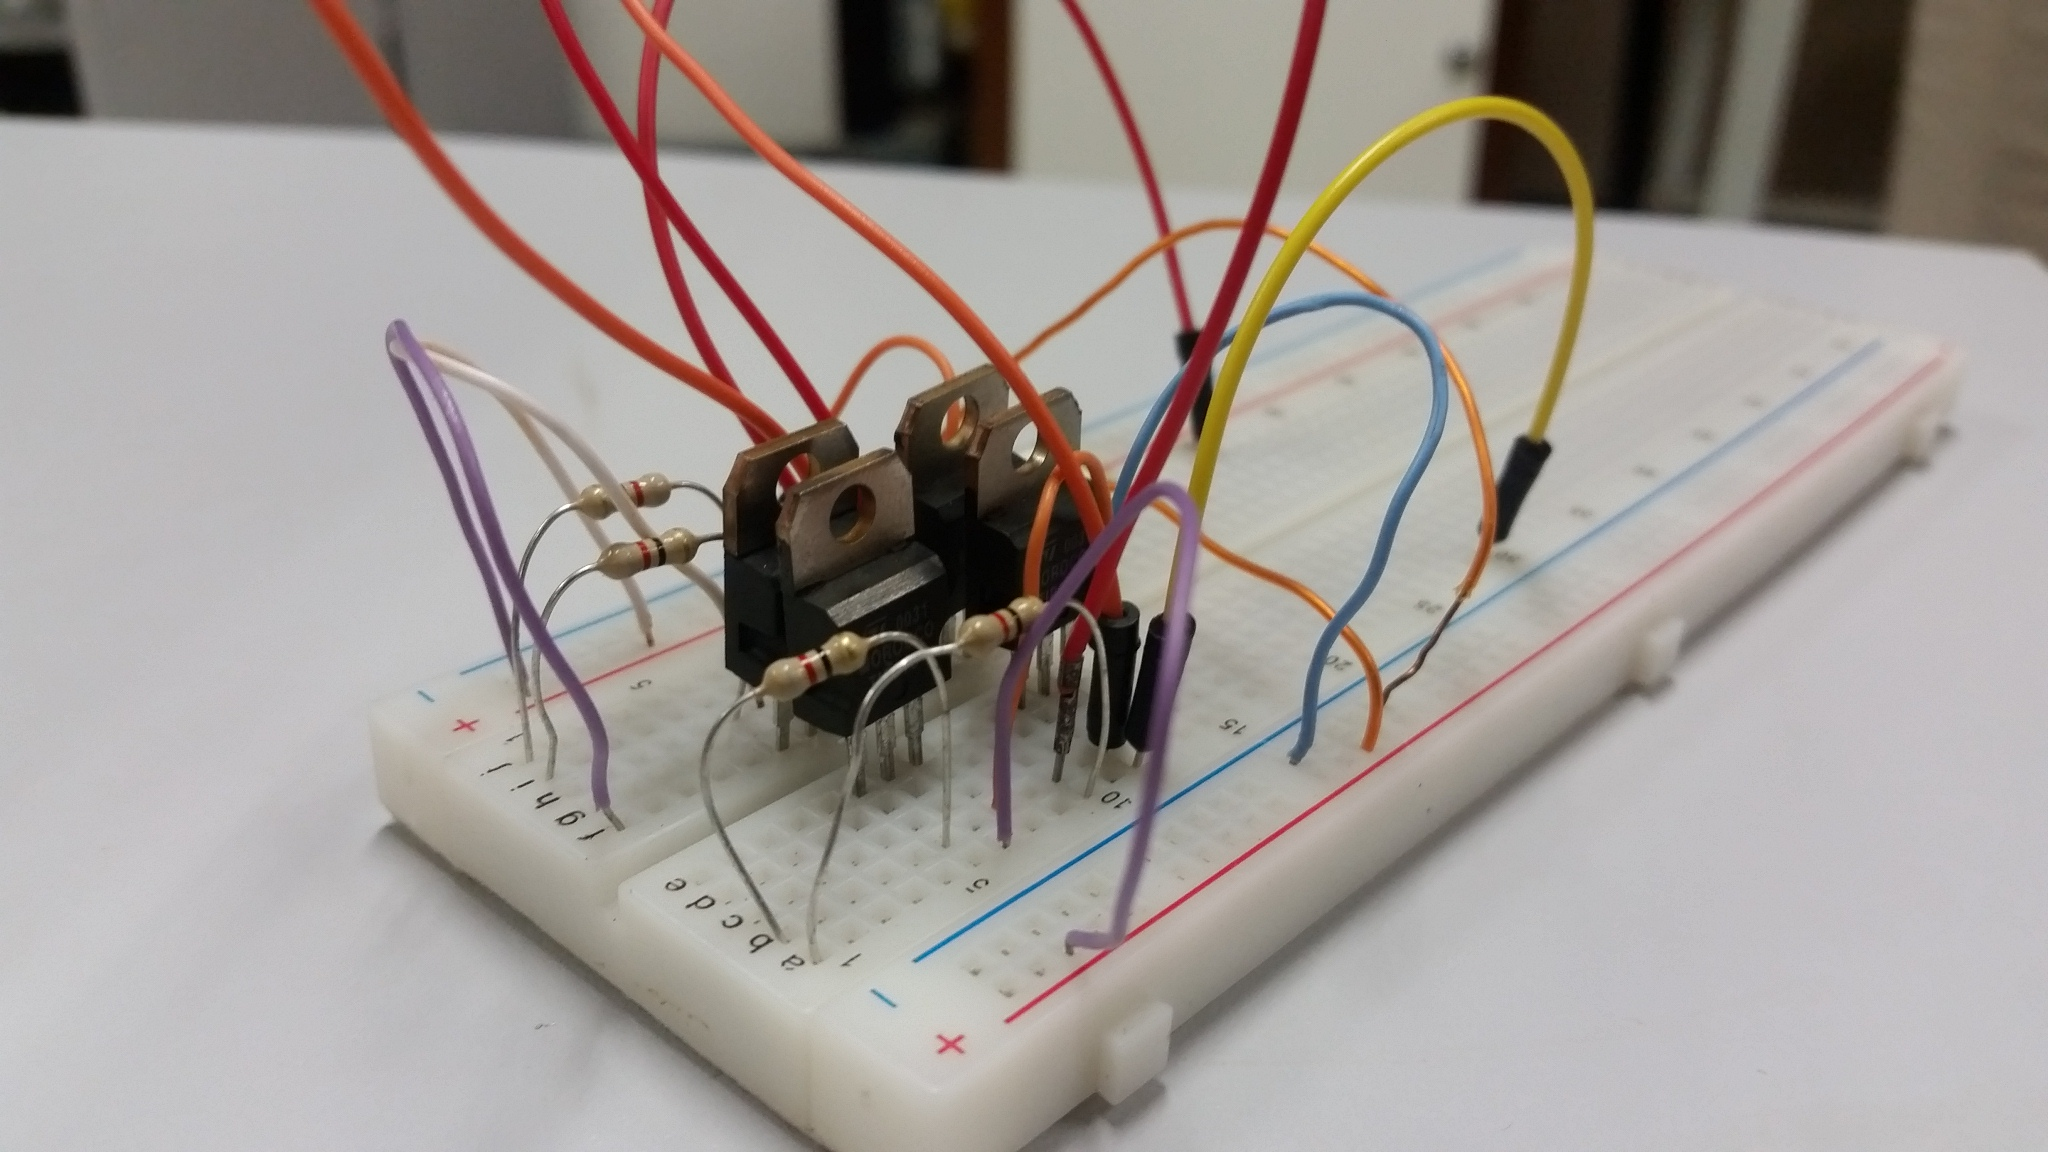
\includegraphics[height=4cm]{img/h_bridge_proto_close.jpg}
\caption{Circuit assembled on a breadboard.}
\label{fig:proto_h}
\end{subfigure}

\begin{subfigure}{.45\columnwidth}
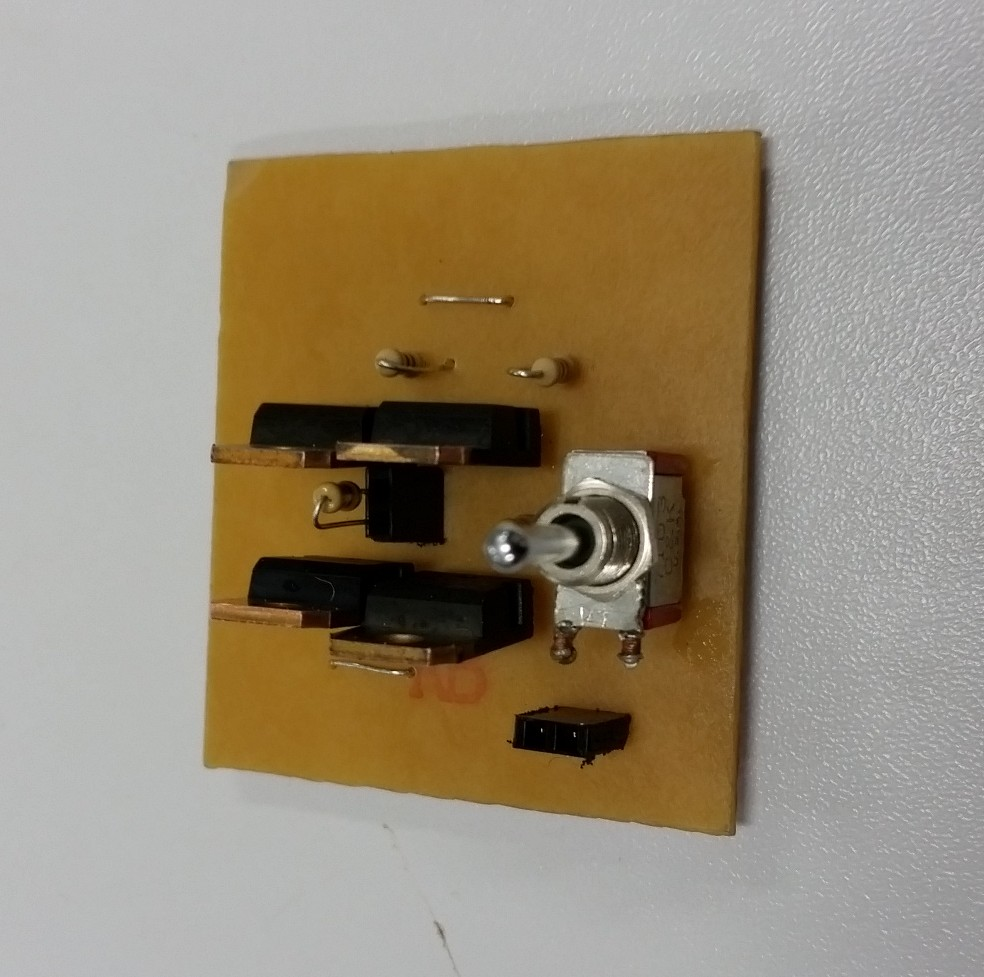
\includegraphics[height=4cm]{img/compontentes4.jpg}
\caption{Components in the PCB.}
\label{fig:pcb_top}
\end{subfigure}
\begin{subfigure}{.45\columnwidth}
\centering
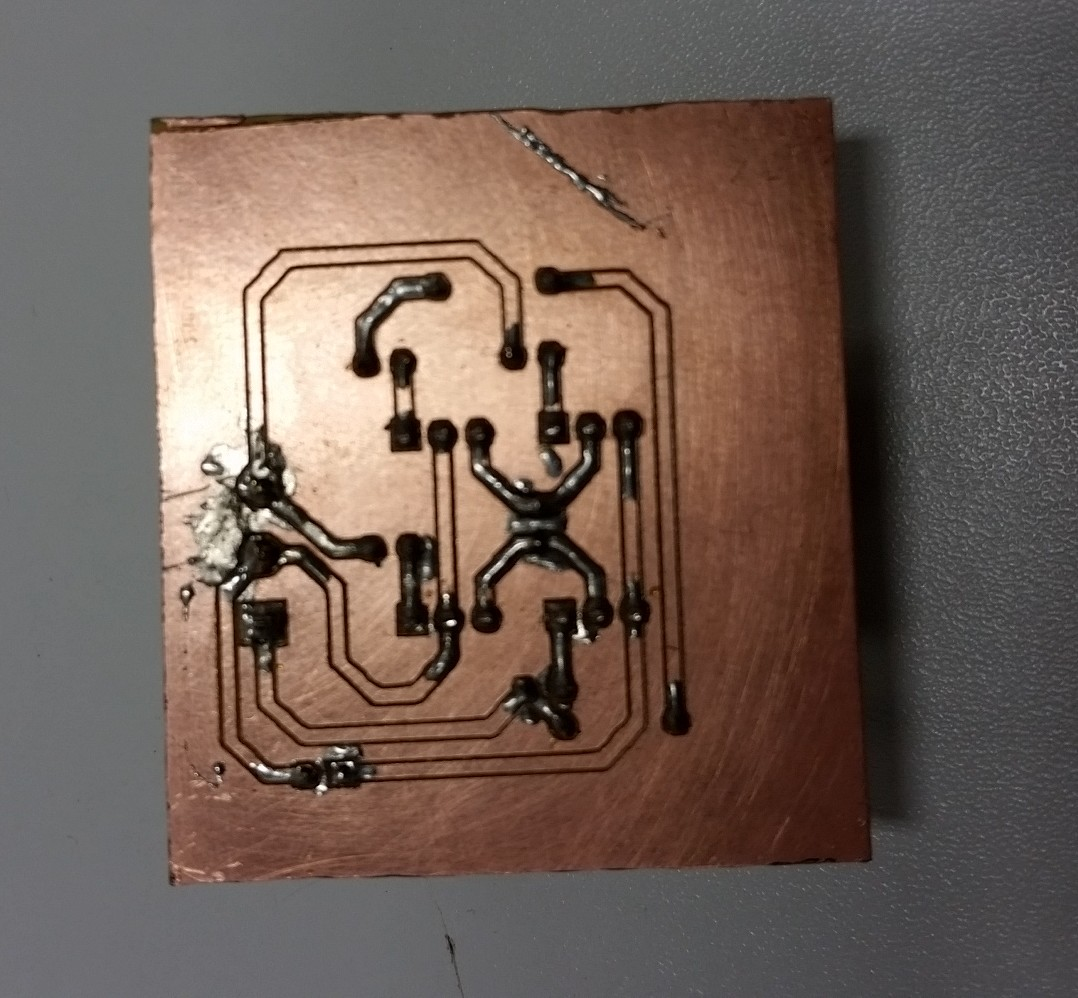
\includegraphics[height=4cm]{img/solda_ja_saiu_da_jaula.jpg}
\caption{Connections in the PCB.}
\label{fig:pcb_bot}
\end{subfigure}

\caption{Circuit assembling.}
\end{figure}
